\documentclass[11pt]{article}
\usepackage[textwidth=18.0cm, textheight=23.0cm, top=2.0cm]{geometry}
\usepackage{pst-all}
\usepackage{amssymb}
\usepackage{tikz}
\usepackage{underscore}\begin{document}
\pagestyle{empty}


ClassName: \underline{\textbf{Class_07.2bp-12}}
\par
BinSize: \underline{\textbf{100 × 100}}
\par
ReduceSize: \underline{\textbf{100 × 100}}
\par
TypeNum: \underline{\textbf{40}}
\par
Num: \underline{\textbf{40}}
\par
OutS: \underline{\textbf{100000}}
\par
InS: \underline{\textbf{83209}}
\par
Rate: \underline{\textbf{0.832}}
\par
UB: \underline{\textbf{10}}
\par
LB0: \underline{\textbf{9}}
\par
LB: \underline{\textbf{10}}
\par
LBWithCut: \underline{\textbf{10}}
\par
NodeCut: \underline{\textbf{0}}
\par
ExtendedNodeCnt: \underline{\textbf{1}}
\par
GenNodeCnt: \underline{\textbf{1}}
\par
PrimalNode: \underline{\textbf{0}}
\par
ColumnCount: \underline{\textbf{91}}
\par
TotalCutCount: \underline{\textbf{0}}
\par
RootCutCount: \underline{\textbf{0}}
\par
LPSolverCnt: \underline{\textbf{82}}
\par
PricingSolverCnt: \underline{\textbf{82}}
\par
BranchAndBoundNum: \underline{\textbf{1}}
\par
isOpt: \underline{\textbf{false}}
\par
TimeOnInitSolution: \underline{\textbf{600.000 s}}
\par
TimeOnPrimal: \underline{\textbf{0.000 s}}
\par
TimeOnPricing: \underline{\textbf{2999.575 s}}
\par
TimeOnRmp: \underline{\textbf{0.112 s}}
\par
TotalTime: \underline{\textbf{3600.007 s}}
\par
\newpage


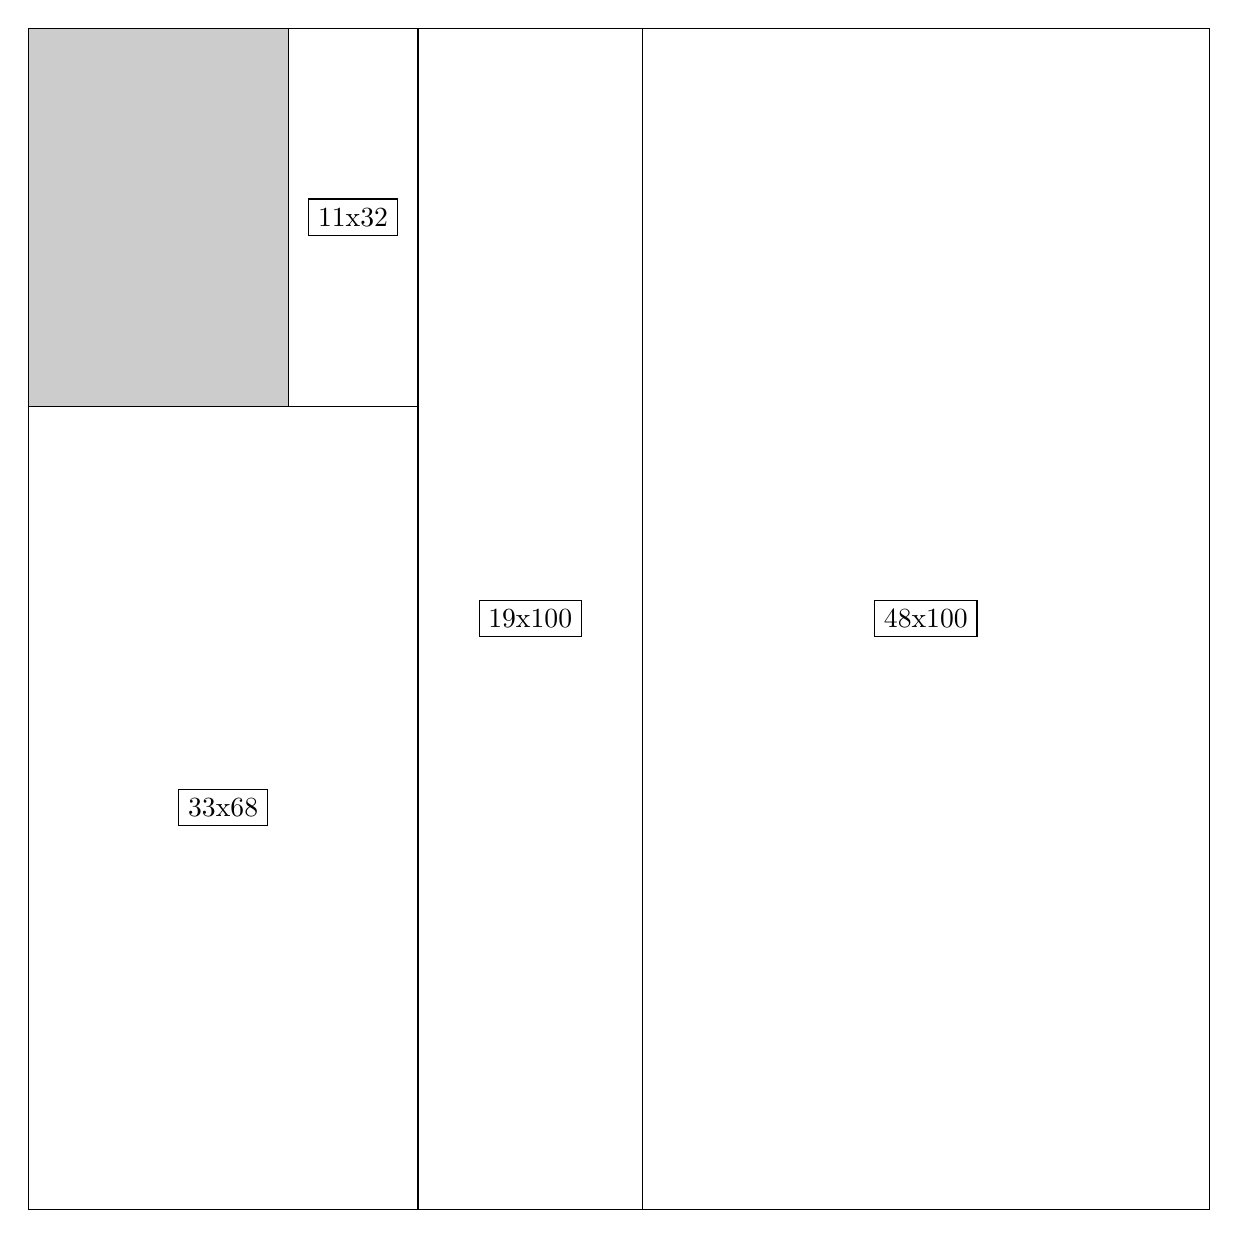
\begin{tikzpicture}[shorten >=1pt,scale=1.0,every node/.style={scale=1.0},->]
\tikzstyle{vertex}=[circle,fill=black!25,minimum size=14pt,inner sep=0pt]
\filldraw[fill=gray!40!white, draw=black] (0,0) rectangle (15.0,15.0);
\foreach \name/\x/\y/\w/\h in {48x100/7.8/0.0/7.199999999999999/15.0,19x100/4.95/0.0/2.85/15.0,33x68/0.0/0.0/4.95/10.2,11x32/3.3/10.2/1.65/4.8}
\filldraw[fill=white!40!white, draw=black] (\x,\y) rectangle node[draw] (\name) {\name} ++(\w,\h);
\end{tikzpicture}


w =48 , h =100 , x =52 , y =0 , v =4800
\par
w =19 , h =100 , x =33 , y =0 , v =1900
\par
w =33 , h =68 , x =0 , y =0 , v =2244
\par
w =11 , h =32 , x =22 , y =68 , v =352
\par
\newpage


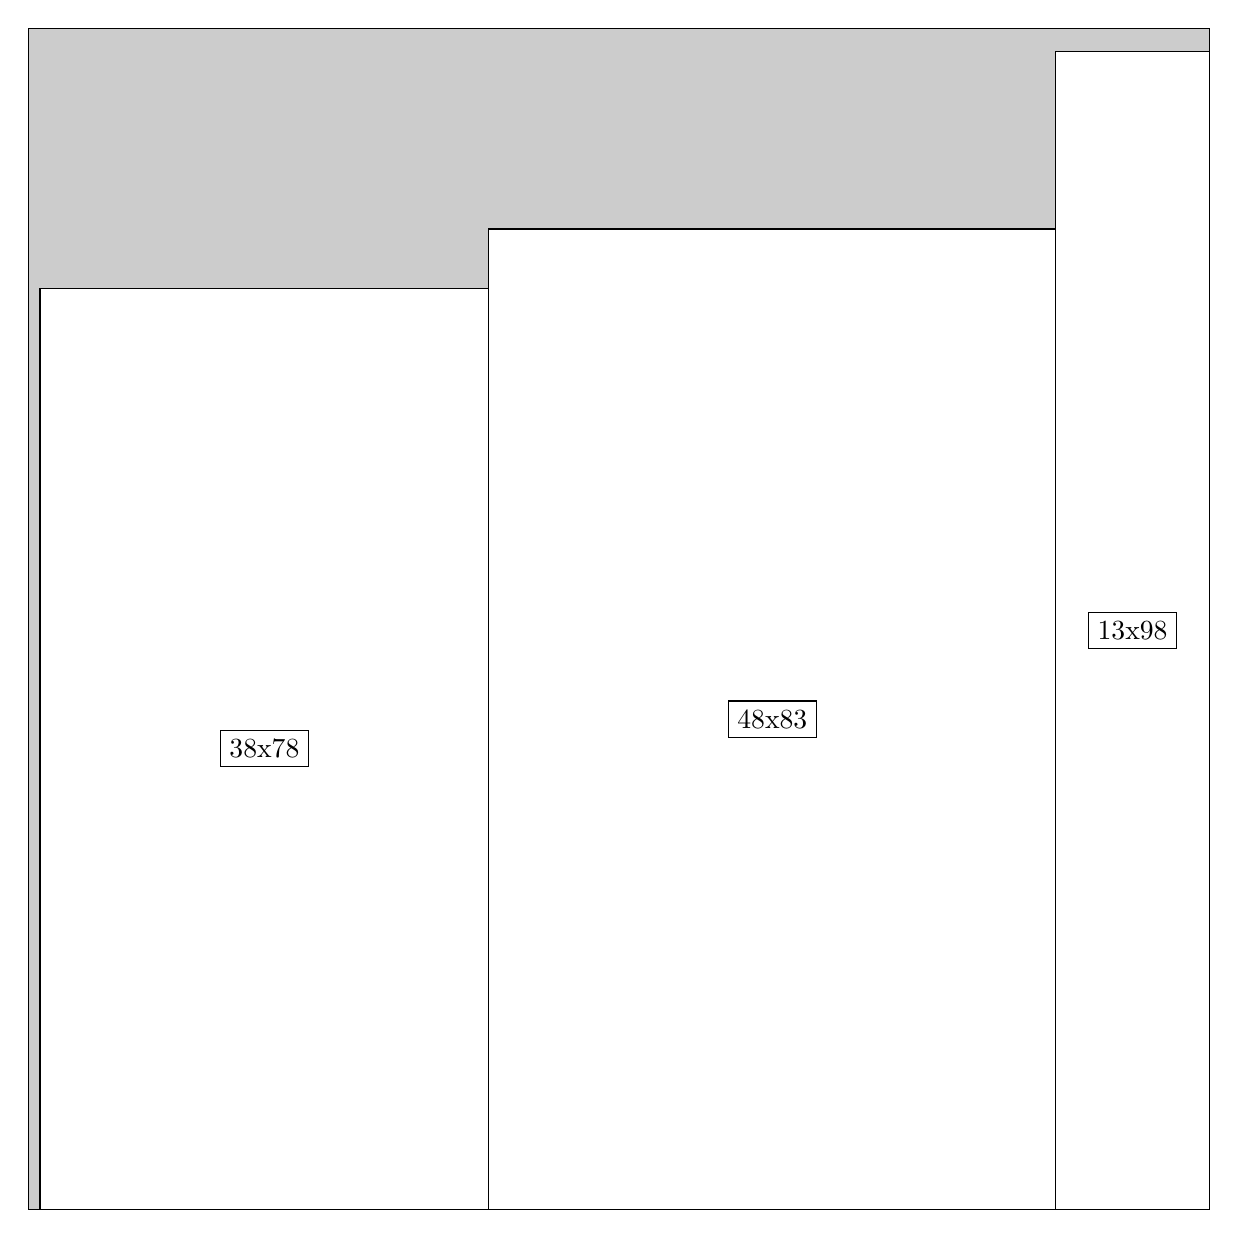
\begin{tikzpicture}[shorten >=1pt,scale=1.0,every node/.style={scale=1.0},->]
\tikzstyle{vertex}=[circle,fill=black!25,minimum size=14pt,inner sep=0pt]
\filldraw[fill=gray!40!white, draw=black] (0,0) rectangle (15.0,15.0);
\foreach \name/\x/\y/\w/\h in {13x98/13.049999999999999/0.0/1.95/14.7,48x83/5.85/0.0/7.199999999999999/12.45,38x78/0.15/0.0/5.7/11.7}
\filldraw[fill=white!40!white, draw=black] (\x,\y) rectangle node[draw] (\name) {\name} ++(\w,\h);
\end{tikzpicture}


w =13 , h =98 , x =87 , y =0 , v =1274
\par
w =48 , h =83 , x =39 , y =0 , v =3984
\par
w =38 , h =78 , x =1 , y =0 , v =2964
\par
\newpage


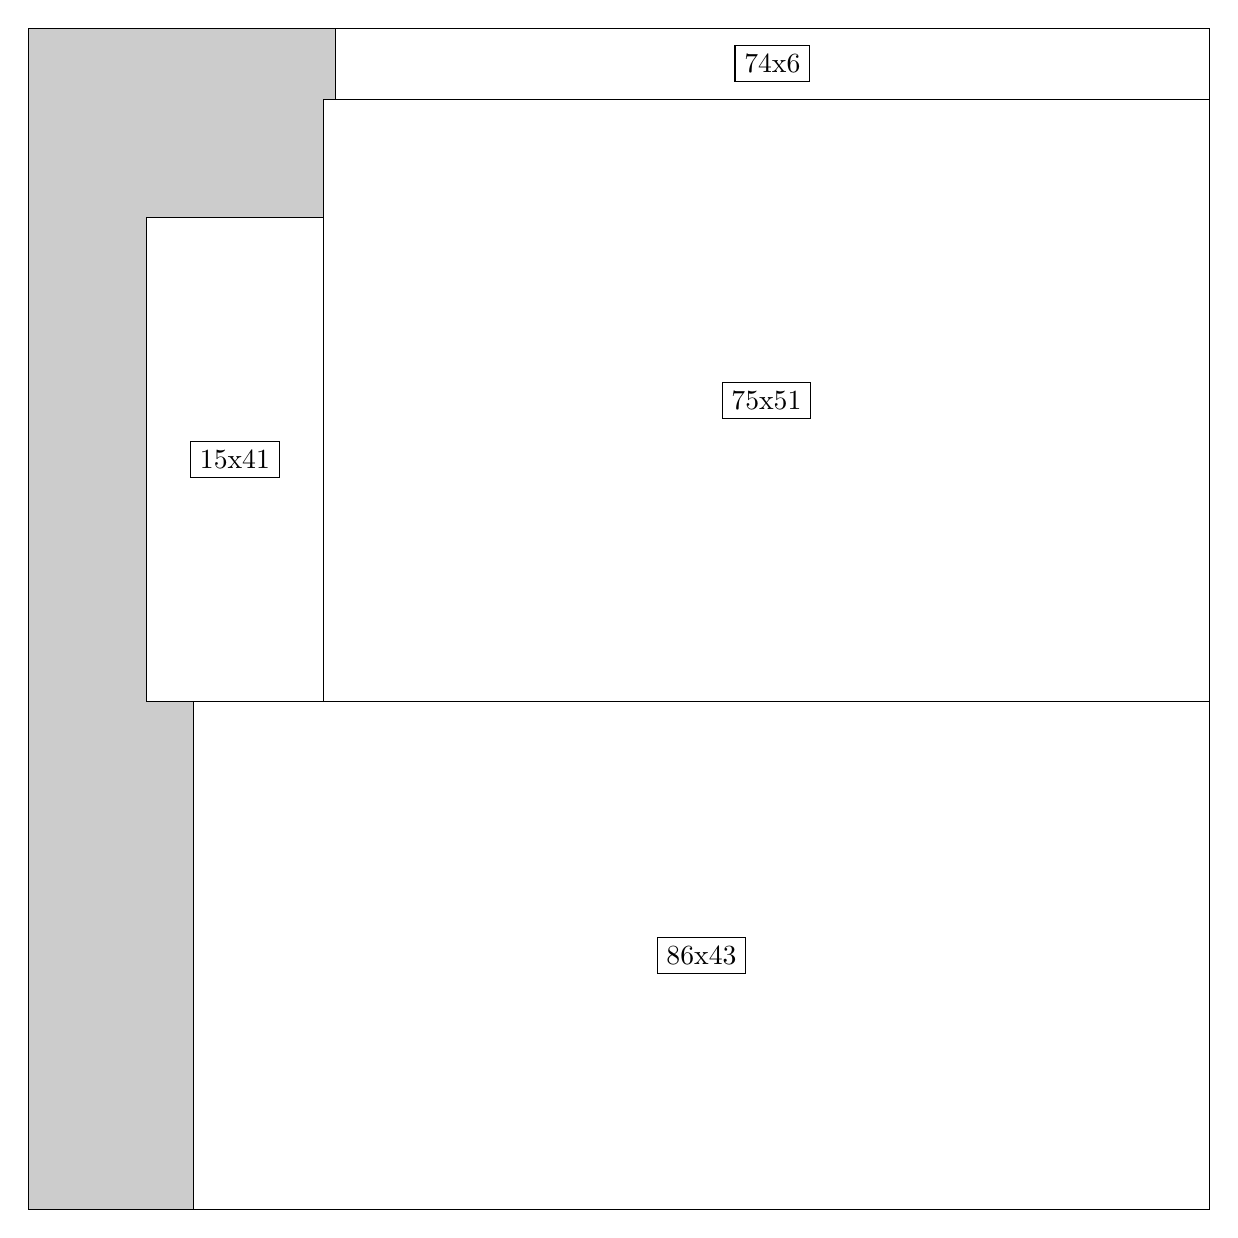
\begin{tikzpicture}[shorten >=1pt,scale=1.0,every node/.style={scale=1.0},->]
\tikzstyle{vertex}=[circle,fill=black!25,minimum size=14pt,inner sep=0pt]
\filldraw[fill=gray!40!white, draw=black] (0,0) rectangle (15.0,15.0);
\foreach \name/\x/\y/\w/\h in {86x43/2.1/0.0/12.9/6.45,75x51/3.75/6.45/11.25/7.6499999999999995,74x6/3.9/14.1/11.1/0.8999999999999999,15x41/1.5/6.45/2.25/6.1499999999999995}
\filldraw[fill=white!40!white, draw=black] (\x,\y) rectangle node[draw] (\name) {\name} ++(\w,\h);
\end{tikzpicture}


w =86 , h =43 , x =14 , y =0 , v =3698
\par
w =75 , h =51 , x =25 , y =43 , v =3825
\par
w =74 , h =6 , x =26 , y =94 , v =444
\par
w =15 , h =41 , x =10 , y =43 , v =615
\par
\newpage


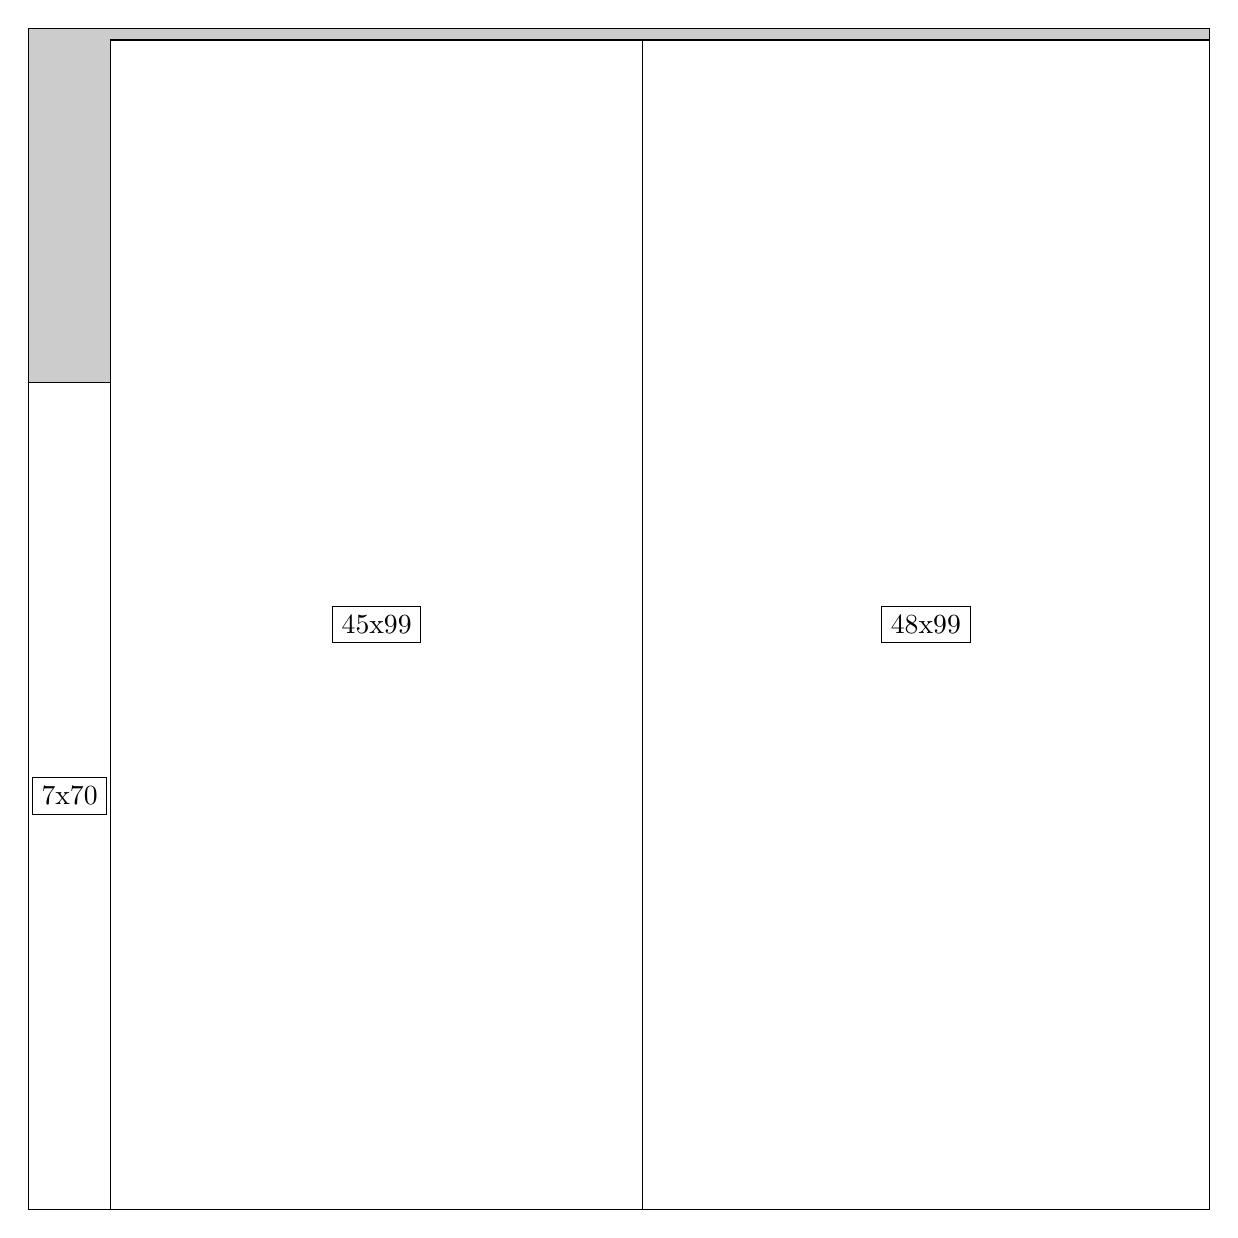
\begin{tikzpicture}[shorten >=1pt,scale=1.0,every node/.style={scale=1.0},->]
\tikzstyle{vertex}=[circle,fill=black!25,minimum size=14pt,inner sep=0pt]
\filldraw[fill=gray!40!white, draw=black] (0,0) rectangle (15.0,15.0);
\foreach \name/\x/\y/\w/\h in {48x99/7.8/0.0/7.199999999999999/14.85,45x99/1.05/0.0/6.75/14.85,7x70/0.0/0.0/1.05/10.5}
\filldraw[fill=white!40!white, draw=black] (\x,\y) rectangle node[draw] (\name) {\name} ++(\w,\h);
\end{tikzpicture}


w =48 , h =99 , x =52 , y =0 , v =4752
\par
w =45 , h =99 , x =7 , y =0 , v =4455
\par
w =7 , h =70 , x =0 , y =0 , v =490
\par
\newpage


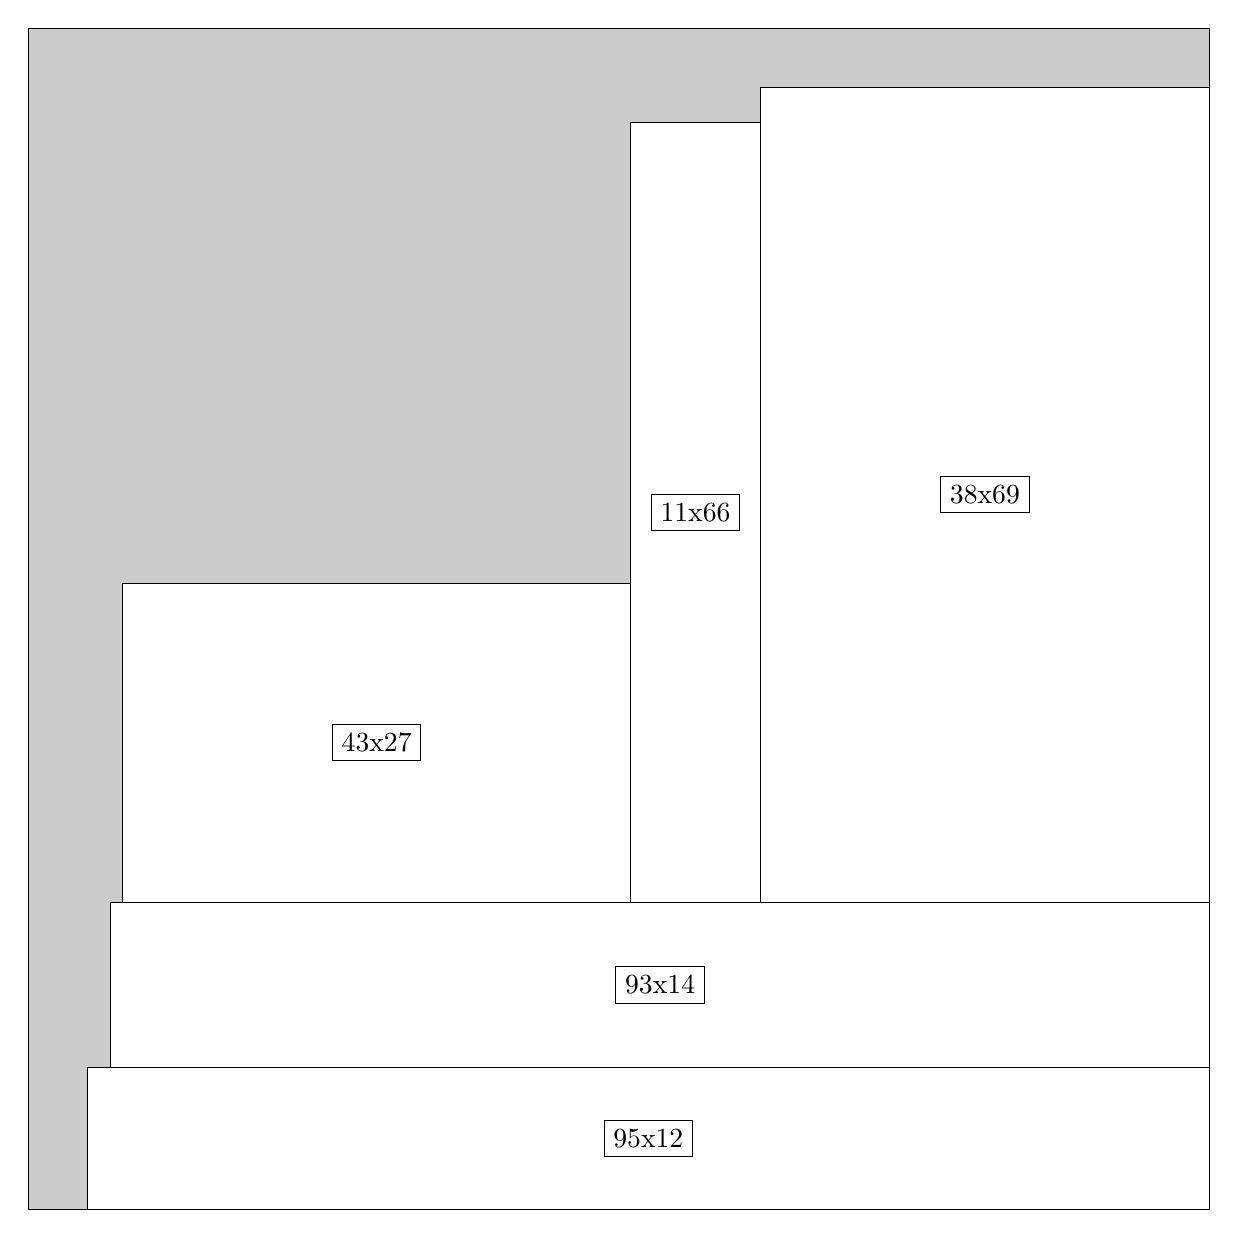
\begin{tikzpicture}[shorten >=1pt,scale=1.0,every node/.style={scale=1.0},->]
\tikzstyle{vertex}=[circle,fill=black!25,minimum size=14pt,inner sep=0pt]
\filldraw[fill=gray!40!white, draw=black] (0,0) rectangle (15.0,15.0);
\foreach \name/\x/\y/\w/\h in {95x12/0.75/0.0/14.25/1.7999999999999998,93x14/1.05/1.7999999999999998/13.95/2.1,38x69/9.299999999999999/3.9/5.7/10.35,11x66/7.6499999999999995/3.9/1.65/9.9,43x27/1.2/3.9/6.45/4.05}
\filldraw[fill=white!40!white, draw=black] (\x,\y) rectangle node[draw] (\name) {\name} ++(\w,\h);
\end{tikzpicture}


w =95 , h =12 , x =5 , y =0 , v =1140
\par
w =93 , h =14 , x =7 , y =12 , v =1302
\par
w =38 , h =69 , x =62 , y =26 , v =2622
\par
w =11 , h =66 , x =51 , y =26 , v =726
\par
w =43 , h =27 , x =8 , y =26 , v =1161
\par
\newpage


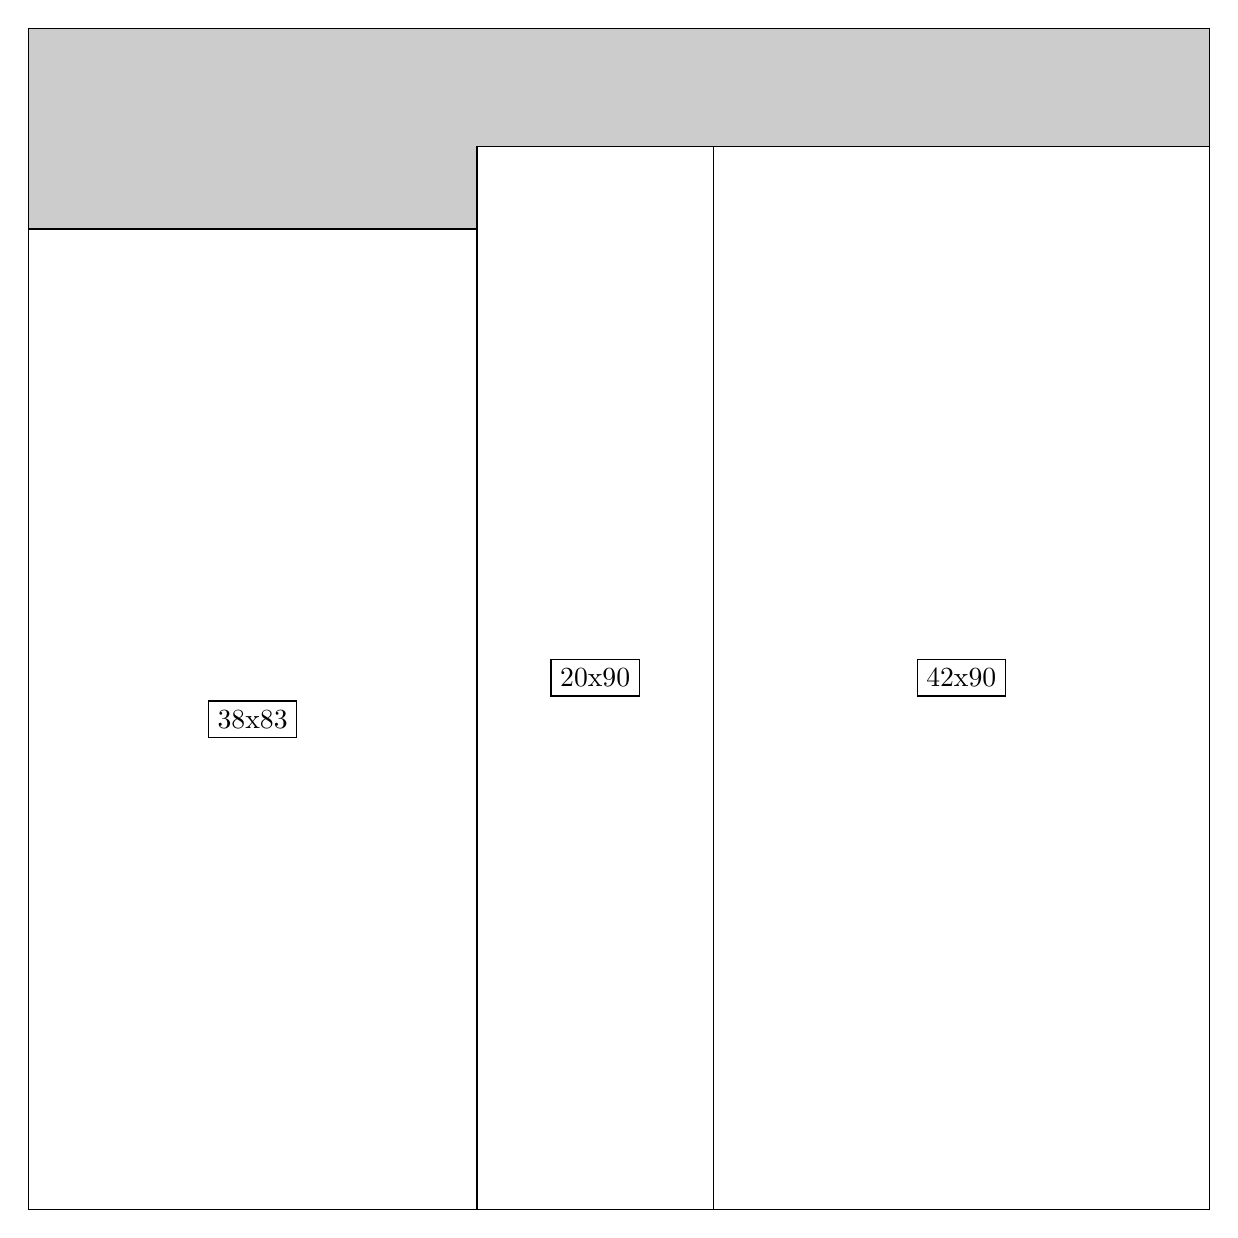
\begin{tikzpicture}[shorten >=1pt,scale=1.0,every node/.style={scale=1.0},->]
\tikzstyle{vertex}=[circle,fill=black!25,minimum size=14pt,inner sep=0pt]
\filldraw[fill=gray!40!white, draw=black] (0,0) rectangle (15.0,15.0);
\foreach \name/\x/\y/\w/\h in {42x90/8.7/0.0/6.3/13.5,20x90/5.7/0.0/3.0/13.5,38x83/0.0/0.0/5.7/12.45}
\filldraw[fill=white!40!white, draw=black] (\x,\y) rectangle node[draw] (\name) {\name} ++(\w,\h);
\end{tikzpicture}


w =42 , h =90 , x =58 , y =0 , v =3780
\par
w =20 , h =90 , x =38 , y =0 , v =1800
\par
w =38 , h =83 , x =0 , y =0 , v =3154
\par
\newpage


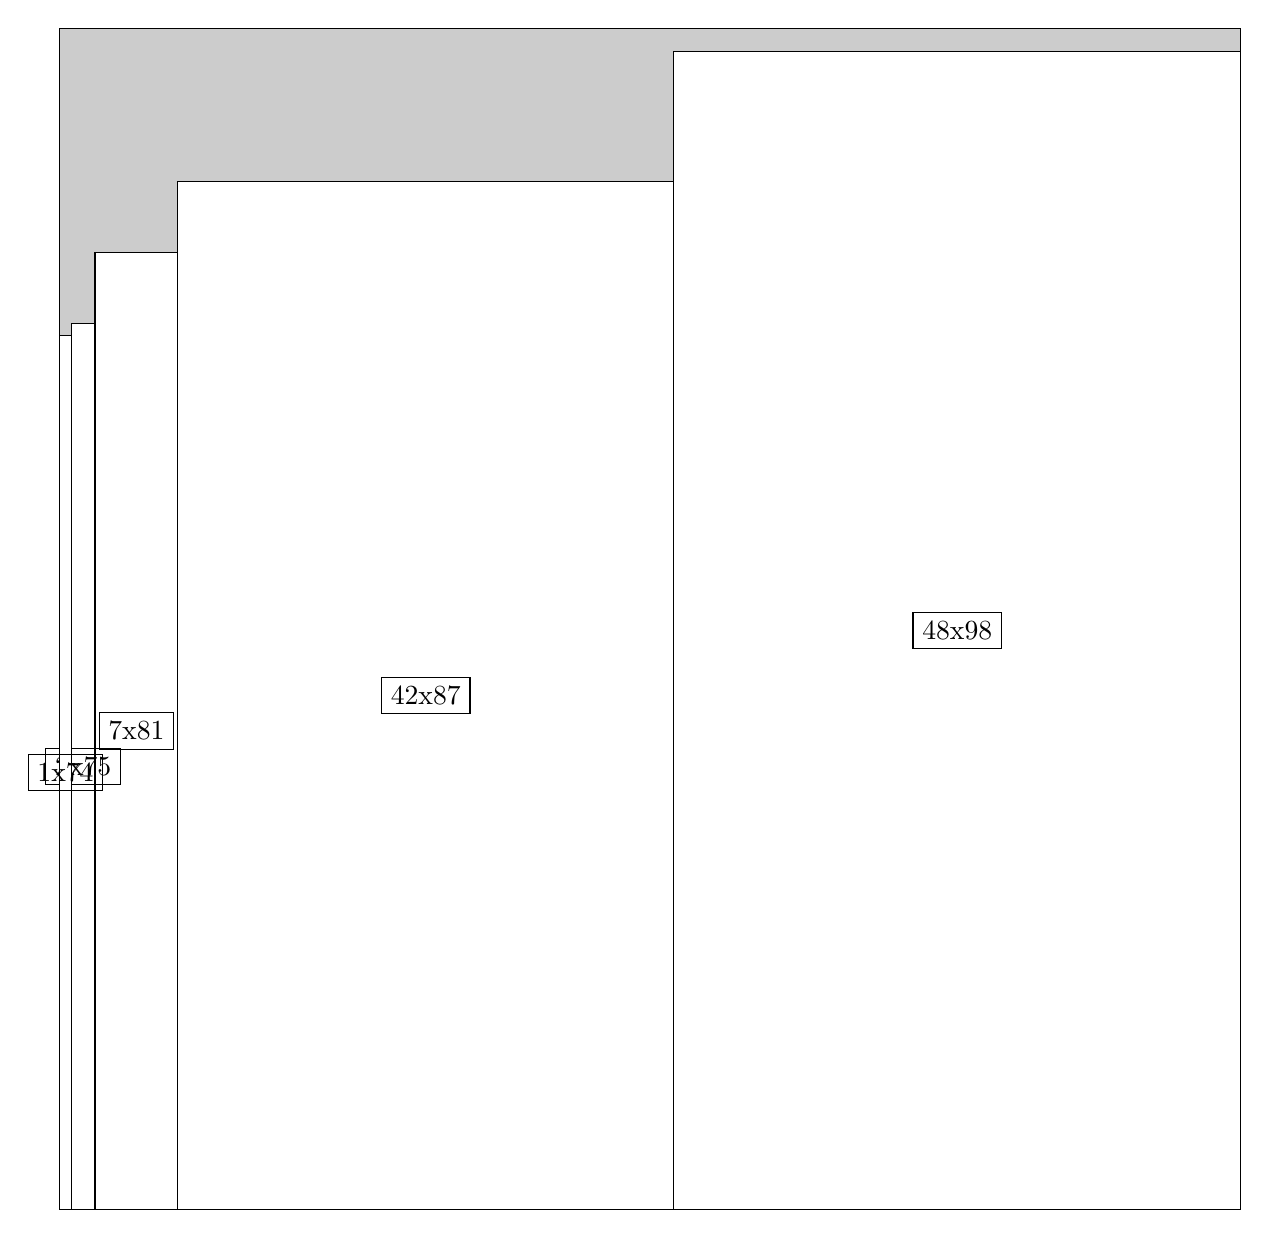
\begin{tikzpicture}[shorten >=1pt,scale=1.0,every node/.style={scale=1.0},->]
\tikzstyle{vertex}=[circle,fill=black!25,minimum size=14pt,inner sep=0pt]
\filldraw[fill=gray!40!white, draw=black] (0,0) rectangle (15.0,15.0);
\foreach \name/\x/\y/\w/\h in {48x98/7.8/0.0/7.199999999999999/14.7,42x87/1.5/0.0/6.3/13.049999999999999,7x81/0.44999999999999996/0.0/1.05/12.15,2x75/0.15/0.0/0.3/11.25,1x74/0.0/0.0/0.15/11.1}
\filldraw[fill=white!40!white, draw=black] (\x,\y) rectangle node[draw] (\name) {\name} ++(\w,\h);
\end{tikzpicture}


w =48 , h =98 , x =52 , y =0 , v =4704
\par
w =42 , h =87 , x =10 , y =0 , v =3654
\par
w =7 , h =81 , x =3 , y =0 , v =567
\par
w =2 , h =75 , x =1 , y =0 , v =150
\par
w =1 , h =74 , x =0 , y =0 , v =74
\par
\newpage


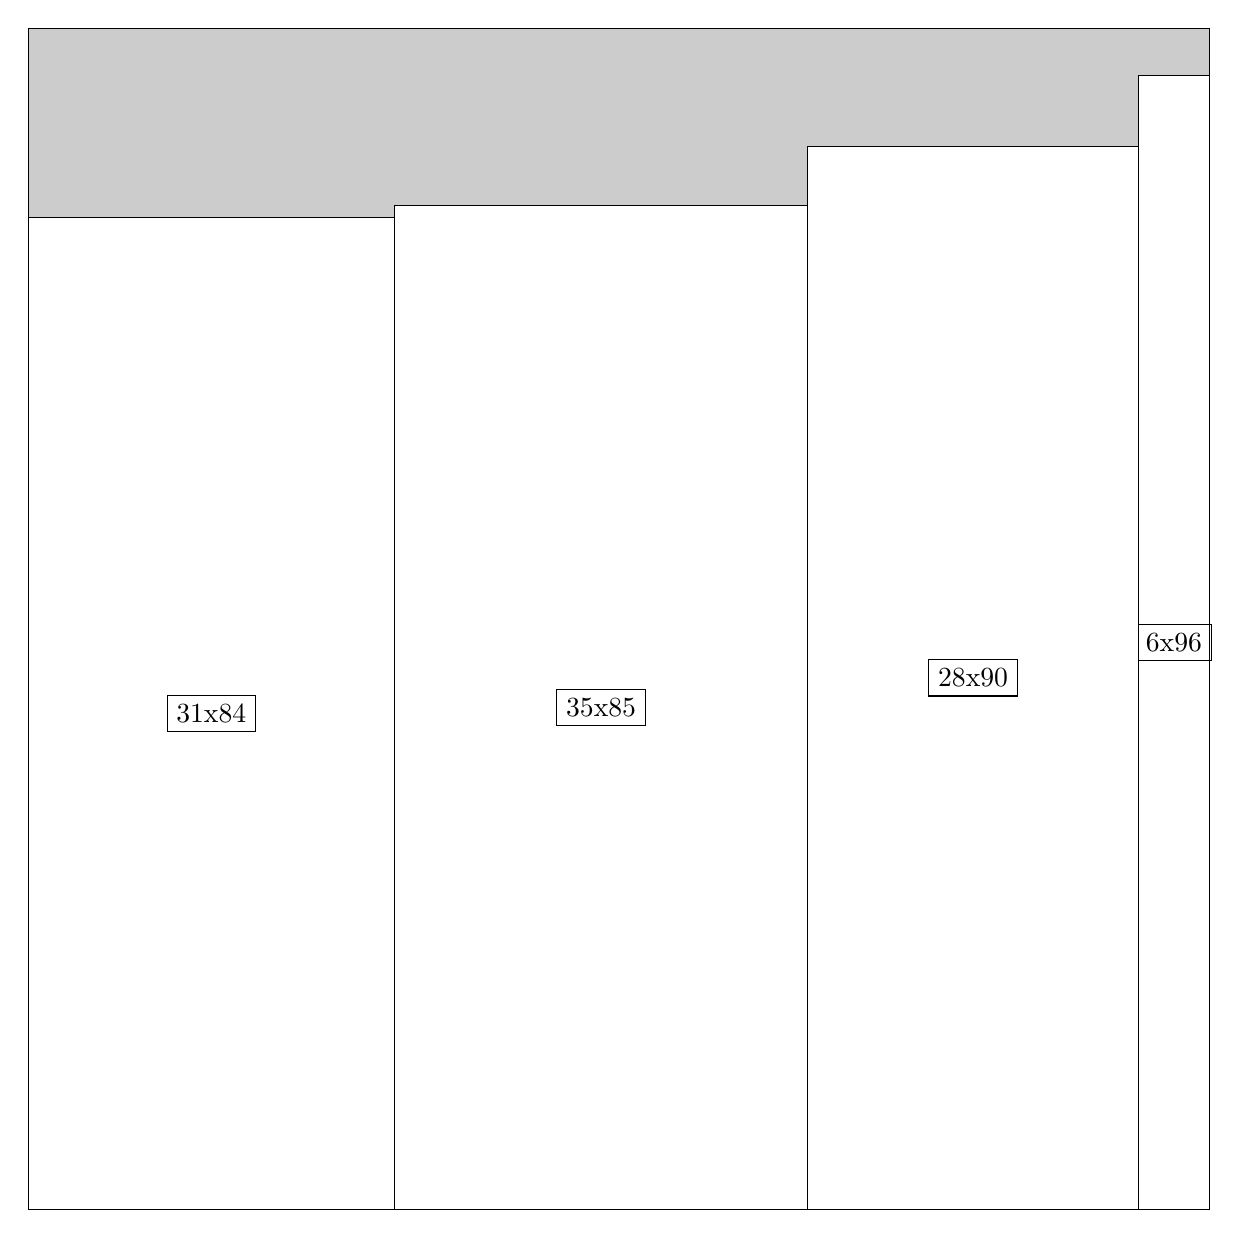
\begin{tikzpicture}[shorten >=1pt,scale=1.0,every node/.style={scale=1.0},->]
\tikzstyle{vertex}=[circle,fill=black!25,minimum size=14pt,inner sep=0pt]
\filldraw[fill=gray!40!white, draw=black] (0,0) rectangle (15.0,15.0);
\foreach \name/\x/\y/\w/\h in {6x96/14.1/0.0/0.8999999999999999/14.399999999999999,28x90/9.9/0.0/4.2/13.5,35x85/4.6499999999999995/0.0/5.25/12.75,31x84/0.0/0.0/4.6499999999999995/12.6}
\filldraw[fill=white!40!white, draw=black] (\x,\y) rectangle node[draw] (\name) {\name} ++(\w,\h);
\end{tikzpicture}


w =6 , h =96 , x =94 , y =0 , v =576
\par
w =28 , h =90 , x =66 , y =0 , v =2520
\par
w =35 , h =85 , x =31 , y =0 , v =2975
\par
w =31 , h =84 , x =0 , y =0 , v =2604
\par
\newpage


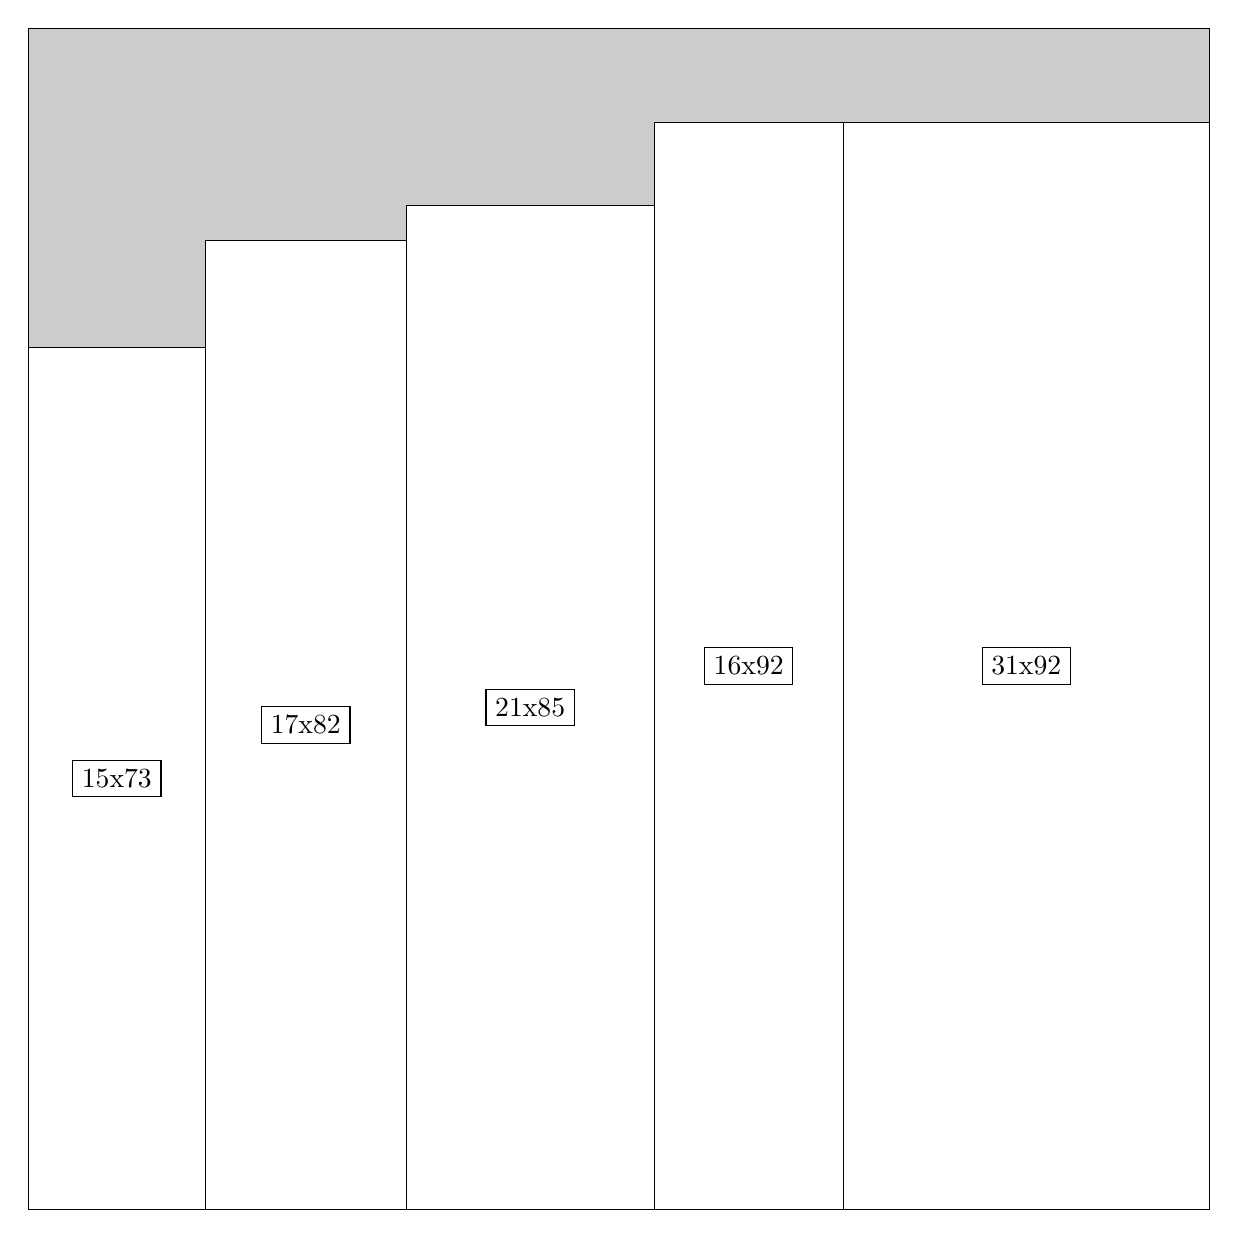
\begin{tikzpicture}[shorten >=1pt,scale=1.0,every node/.style={scale=1.0},->]
\tikzstyle{vertex}=[circle,fill=black!25,minimum size=14pt,inner sep=0pt]
\filldraw[fill=gray!40!white, draw=black] (0,0) rectangle (15.0,15.0);
\foreach \name/\x/\y/\w/\h in {31x92/10.35/0.0/4.6499999999999995/13.799999999999999,16x92/7.949999999999999/0.0/2.4/13.799999999999999,21x85/4.8/0.0/3.15/12.75,17x82/2.25/0.0/2.55/12.299999999999999,15x73/0.0/0.0/2.25/10.95}
\filldraw[fill=white!40!white, draw=black] (\x,\y) rectangle node[draw] (\name) {\name} ++(\w,\h);
\end{tikzpicture}


w =31 , h =92 , x =69 , y =0 , v =2852
\par
w =16 , h =92 , x =53 , y =0 , v =1472
\par
w =21 , h =85 , x =32 , y =0 , v =1785
\par
w =17 , h =82 , x =15 , y =0 , v =1394
\par
w =15 , h =73 , x =0 , y =0 , v =1095
\par
\newpage


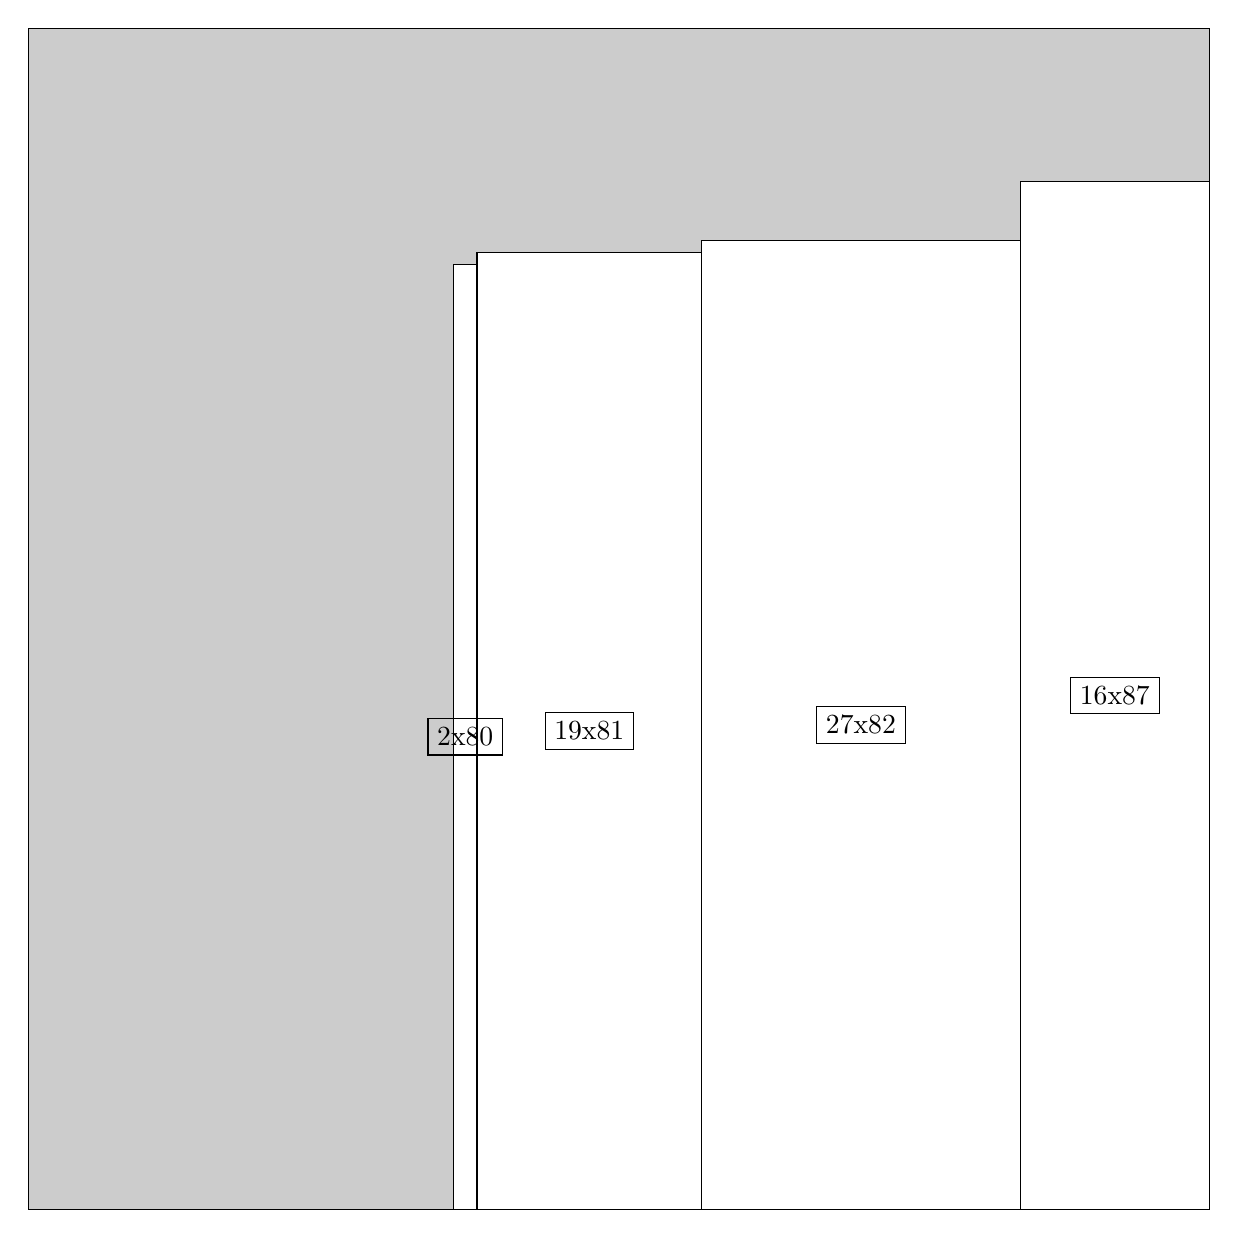
\begin{tikzpicture}[shorten >=1pt,scale=1.0,every node/.style={scale=1.0},->]
\tikzstyle{vertex}=[circle,fill=black!25,minimum size=14pt,inner sep=0pt]
\filldraw[fill=gray!40!white, draw=black] (0,0) rectangle (15.0,15.0);
\foreach \name/\x/\y/\w/\h in {16x87/12.6/0.0/2.4/13.049999999999999,27x82/8.549999999999999/0.0/4.05/12.299999999999999,19x81/5.7/0.0/2.85/12.15,2x80/5.3999999999999995/0.0/0.3/12.0}
\filldraw[fill=white!40!white, draw=black] (\x,\y) rectangle node[draw] (\name) {\name} ++(\w,\h);
\end{tikzpicture}


w =16 , h =87 , x =84 , y =0 , v =1392
\par
w =27 , h =82 , x =57 , y =0 , v =2214
\par
w =19 , h =81 , x =38 , y =0 , v =1539
\par
w =2 , h =80 , x =36 , y =0 , v =160
\par
\newpage


\end{document}